% Lecture file created by Gemini
% Class: Quantum Information With Atoms and Photons
% Professor: Pietro Silvi
% Date: 2025-10-16
\lecture{5}{Lifting atom degeneracy}{2025-10-16}

% --- Start writing here ---
\captionsetup{singlelinecheck=false}
Lifting Energy-Level degeneracies in Hydrogen-like atoms

NOU RELATNISTIC $>H=\frac{\vec{p}^{2}}{2 m}+V_{\text {egr }}$ (OUI)

$$
\begin{aligned}
& m \approx m_{e} \quad \text { RESUCES MASS } \\
& {\left[T_{3}, P_{1}\right]=i \hbar \delta_{11} \quad \text { RESOCES }} \\
& \text { COORS-MOM. }
\end{aligned}
$$

True\\
HYDROGEN\\
energy levels\\
energy levels\\
$V(\Omega)=-\frac{(z=1) e^{2}}{4 \pi \varepsilon_{0}} \frac{1}{2} \quad V(\Omega)=-\frac{(z=1) e^{2}}{4 \pi \varepsilon_{0}}\left(\frac{1}{2}+C(\Omega)\right) \quad V(\Omega)=-\frac{(z=2) e^{2}}{4 \pi \varepsilon_{0}}$\\
$\xrightarrow{\text { ENERGY LEVELS }} E_{n(e)}=-\frac{m_{e} e^{4} z_{k}^{2}}{2\left(4 \pi \varepsilon_{0}\right)^{2} \hbar^{2}}\left(\frac{1}{n^{2}}+\widetilde{\zeta}_{n, e}\right)$\\
$\uparrow \Rightarrow L_{\text {corre ction for }}$\\
COMAARING THIS EXPRESSION TO THE ELECTRON REST ENERGY\\
$E_{n(e)}=-\frac{m c^{2}}{2} Z_{R}^{2}(\underbrace{\frac{e^{2}}{4 \pi \varepsilon_{0} \hbar c}}_{\text {Fine Structure }})^{2}\left(\frac{1}{n^{2}}+\zeta_{n, e}\right)=-\frac{m c^{2}}{2}\left(Z_{R} \alpha\right)^{2}(\ldots)$\\
$n c^{2} \approx m_{e} c^{2}=511 \mathrm{KeV} \rightarrow E_{n=1}^{H \times D A O}=-\frac{511 \mathrm{KeV}}{2(137)^{2}}=-13.6 \mathrm{eV}$\\
$E_{n(e)}^{\text {Hol } \mathrm{k} \mathrm{e} \mathrm{e}}=-\frac{m_{e} c^{2}}{2}\left(Z_{R} \alpha\right)^{2}\left(\frac{1}{n^{2}}+\tilde{e}_{n e}\right)$\\
natural alkal $z_{c}=1$\\
AKKALME-EARTH IONS $z_{R}=2$\\
Lifting the Degenerocy.\\[0pt]
(1) Fine structure arsa. spin-orbit coupung [native perturbation]\\
(2) Eeeman Smitting [external $\vec{B}$ static, can de perturbative]

ACKALINE-EARTH\\
IONS\\
$-\frac{(z=2) e^{2}}{4 \pi \varepsilon_{0}}\left(\frac{1}{2}+c(r)\right)$\\
COREECTION AT\\
SHORT RADII lower $e$\\
states of the outer shell electron\\
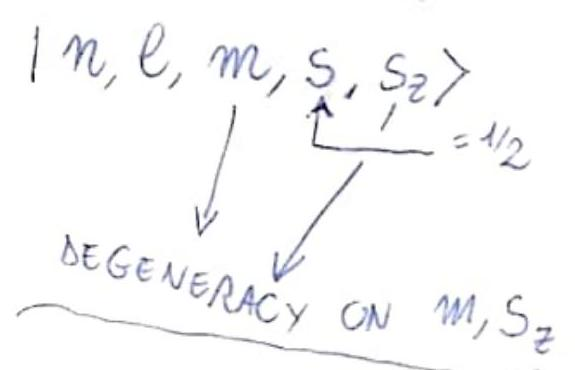
\includegraphics[max width=\textwidth, center]{2025_10_16_e34e240cf6beac2f9e0dg-1}

\section*{Fine Structure (a quick outrview) - lowest orser of $\vec{B}$ fields}
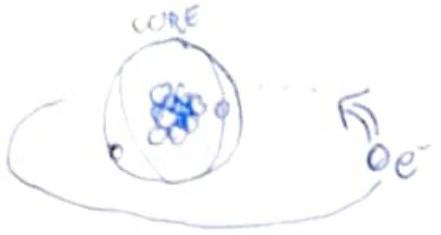
\includegraphics[max width=\textwidth, center]{2025_10_16_e34e240cf6beac2f9e0dg-2(1)}\\
NO MAGNETIC FHELS IN LAB FRAME\\
$\downarrow$\\
yes thageetive fleed in é rest frame\\
$\left.\underset{\uparrow}{\vec{B}}=-\frac{1}{C^{2}} \vec{v} \times \vec{E}=\left\lvert\, \begin{array}{c}\text { CORE } \\ \text { ELECTRIC FIELD } \\ \text { IN LAE FRAME } \\ \text { ELECTRON VELOCITY }\end{array}\right.\right\}$ III ITS REST FRDME

THIS COMES FROM delativity + MAXWELL EQS.\\
$\vec{E}$ is radial so

$$
\vec{E}=\frac{\vec{\nabla} V}{-e}=\frac{t \vec{r}}{e|r|} \partial_{r} V_{\text {elf }} / r
$$

$\vec{B}_{\text {tect }}=-\frac{1}{c^{2}}\left(\frac{\vec{P}}{m} \times \vec{r}\right)\left(+\frac{1}{e r} \frac{\partial V_{e r}}{\partial r}\right)$

BUT

$$
\vec{P} \times \vec{r}=-\vec{r} \times \vec{P}=\vec{L}
$$

even in guantuh mechanic\\
$\vec{B}_{\text {FERT }}=\left(+\frac{1}{\text { emc }{ }^{2} r} \frac{\partial V}{\partial r}\right) \vec{L}_{\text {angular momentul in the las frame }}$

How the é spin has a magnetic DIOCE MCMENT ASSOCIATES TO IT\\
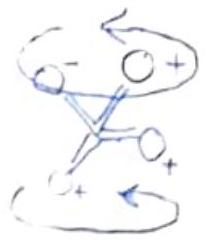
\includegraphics[max width=\textwidth, center]{2025_10_16_e34e240cf6beac2f9e0dg-2(2)}\\
A RIGID SYSTEM CF\\
(SPHERICAUY-SISTRIBUTED) massive charges mas

$$
\vec{\mu}=\frac{9}{2 m} \vec{L}
$$

THIS MOULL FALLS FOR THE EECTRON i.i a. FACTOR ge

$$
\sqrt{415} \text { monell }
$$

$$
\vec{\mu}=-\frac{e}{2 m} g_{S} \vec{S}-\text { SPMGUAR }
$$

\begin{center}
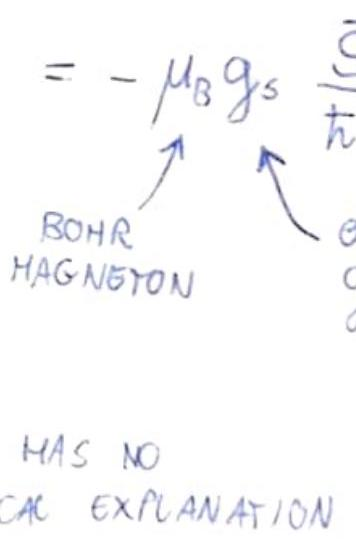
\includegraphics[max width=\textwidth]{2025_10_16_e34e240cf6beac2f9e0dg-2}
\end{center}

$$
\begin{aligned}
& \mu_{B}=\frac{e \hbar}{2 m_{e}} \\
& { }_{O R}
\end{aligned}
$$

olectron

$$
g-\text { FACTOR }
$$

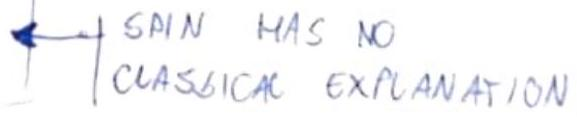
\includegraphics[max width=\textwidth, center]{2025_10_16_e34e240cf6beac2f9e0dg-2(3)}\\
3. $2 \frac{\text { FROM SIRAC FREE THEORY }}{\text { VARIA TI⿴囗 ANY FERMION S=1/2 }}>$ CORRECTIONS?\\
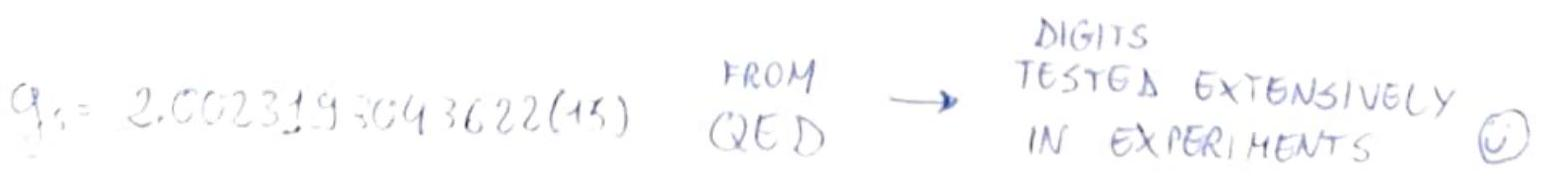
\includegraphics[max width=\textwidth, center]{2025_10_16_e34e240cf6beac2f9e0dg-2(4)}

COUPING $\vec{B}$ TO $\vec{\mu}$\\
$H=-\vec{\mu} \cdot \vec{B} \leftarrow$ SO SIMPLE $\} \begin{aligned} & \text { Precession } \\ & \text { HAHICTONIAN }\end{aligned}$\\
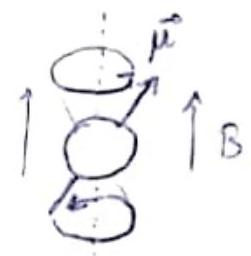
\includegraphics[max width=\textwidth, center]{2025_10_16_e34e240cf6beac2f9e0dg-3}\\
$\left.H\left(\begin{array}{c}\text { ELECTRON } \\ \text { REST } \\ \text { FRAME }\end{array}\right)=-\left(-\frac{\mu_{B} g_{S}}{\hbar}\right) \right\rvert\, \vec{S} \cdot\left(\frac{1}{e_{m c^{2}} r} \frac{\partial V}{\partial r}\right) \vec{L}=$\\
$=+\frac{\mu_{B} g_{s}}{e m c^{2} \hbar}\left(\frac{1}{r} \frac{\partial V_{\text {ess }}}{\partial r}\right) \vec{S} \cdot \vec{L}$ HOWEVER, WE NEED TO MOVE EFFECT $\rightarrow g_{S} \xrightarrow[\text { LAB }]{\text { TO }} g_{S}-1$\\
$H\binom{\text { LAB }}{\text { FRAME }}=\frac{\mu_{B}\left(g_{s}-1\right)}{e m c^{2} \hbar}\left(\frac{1}{2} \frac{\partial V_{\text {eff }}}{\partial r}\right) \vec{S} \cdot \vec{L} \quad\left\{\begin{array}{c}\text { PUGGING Hydeo-LIKE } \\ \text { POTENTIAL } \\ Z_{0} e^{2}(1\end{array}\right. V(r)=-\frac{Z_{R} e^{2}}{4 \pi \varepsilon_{0}}\left(\frac{1}{r}+e(r)\right)$\\
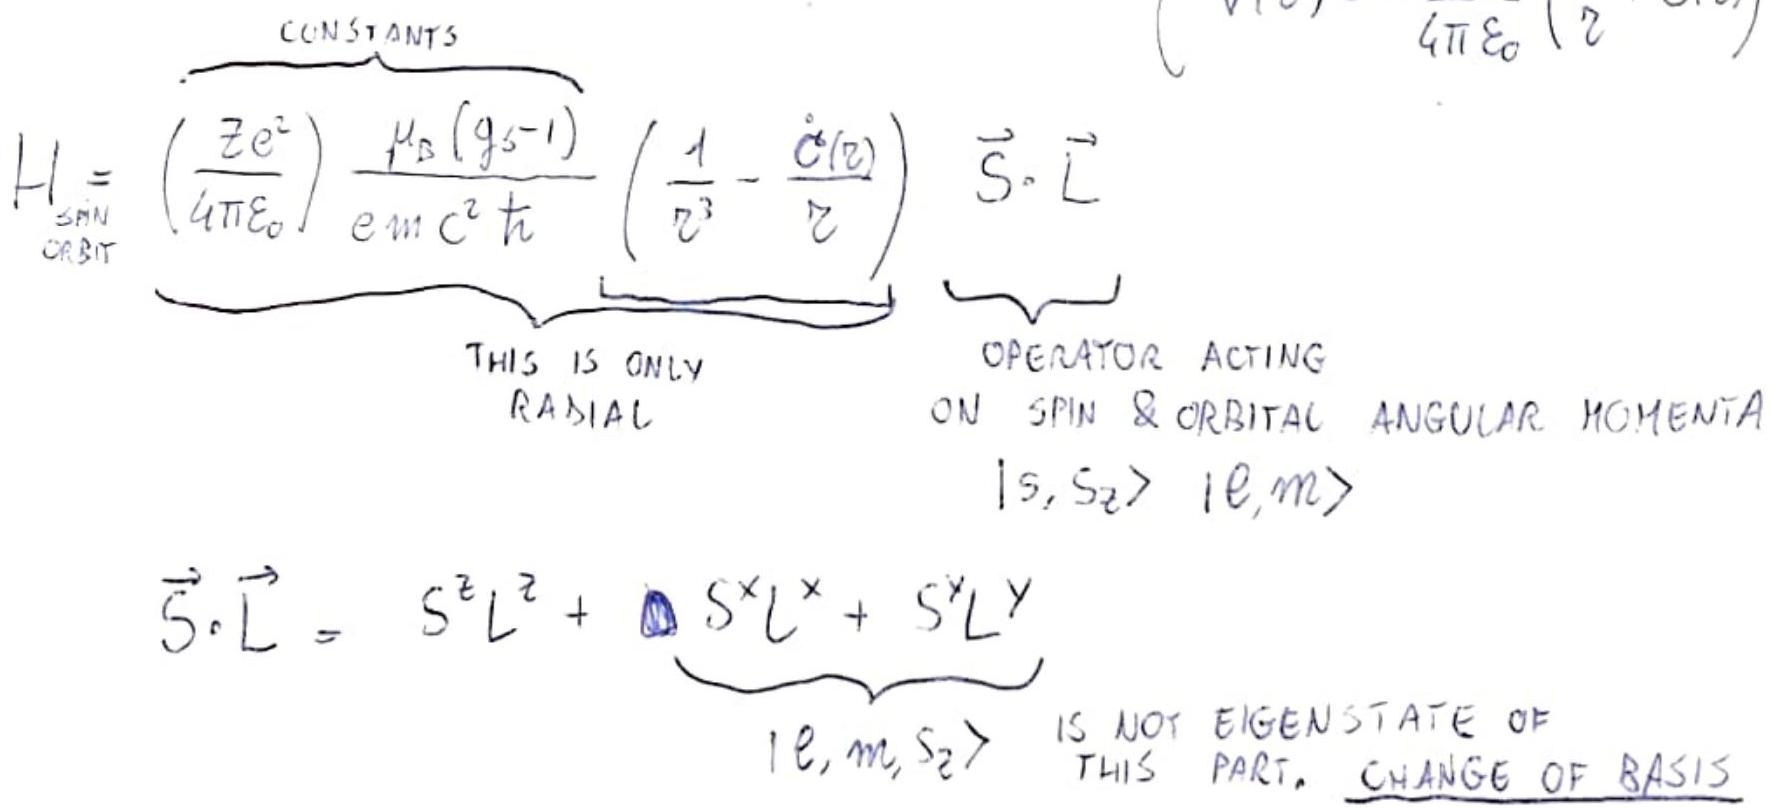
\includegraphics[max width=\textwidth, center]{2025_10_16_e34e240cf6beac2f9e0dg-3(1)}\\
$\vec{J}\left(\frac{\text { TOTAL }}{\begin{array}{l}\text { TOLALAR } \\ \text { MOMENTUM }\end{array}}\right)=\vec{L}+\vec{S}$ SUM OF TWO ANGULAR MOMENTUM OPERATOR ALGEBRAS (OR FUSION)

$$
\begin{aligned}
{\left[J_{J}, J_{K}\right]=\left[L_{J}, L_{K}\right]+\left[L_{J}, S_{K}\right]+\left[S_{K}, L_{J}\right]+\left[S_{1}, S_{K}\right]=} & \\
& i \varepsilon_{j K e} L_{e}+i \varepsilon_{jKe} S_{e}=i \varepsilon_{jKe}(L+S)_{e}=i \varepsilon_{jKl}-J_{e}
\end{aligned}
$$

also in angular momentum

PRODUCT BASIS\\
$\left|e, m ; s, s_{z}\right\rangle$\\
$\rightarrow \underset{\text { UPON }}{\text { BASE }} \quad L^{2}, L_{z}, S^{2}, S_{z} \quad \underset{\text { COMUTINE }}{\text { AU }}$\\
$\left.\left(\begin{array}{l}L^{2} \\ L_{z} \\ s^{2} \\ s_{z}\end{array}\right)\left|l, m ; s, s_{z}\right\rangle=1.\right\rangle\left(\begin{array}{c}\hbar^{2} e(e+1) \\ \hbar m \\ \hbar^{2} s(s+1) \\ \hbar s_{z}\end{array}\right)$

FUSION BASIS\\
$|U, S ; J, J z\rangle$\\
$L \xrightarrow[\substack{\text { BASED } \\ \text { UPON }}]{ } L^{2}, S^{2}, J^{2}, J_{z} \quad$ COMHUTING\\
$\left(\begin{array}{l}L^{2} \\ S^{2} \\ J^{2} \\ J_{z}\end{array}\right) 1_{0}>1 .>\left(\begin{array}{c}\hbar^{2} e(e+1) \\ \hbar^{2} s(s+1) \\ \hbar^{2} J(J+1) \\ \hbar J z\end{array}\right)$\\
EXAMPLE $l=2$\\
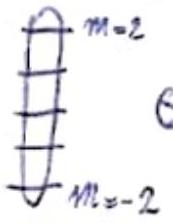
\includegraphics[max width=\textwidth, center]{2025_10_16_e34e240cf6beac2f9e0dg-4}\\
(2) $\theta_{S_{z}=-1 / 2}^{S_{z}+1 / 2} \quad \begin{gathered}D \times 2=10 \\ 5 \times 2\end{gathered}$\\
il FUSES into $\oplus$ J-SPACES FROM $|l-s|$ TO $l+s \quad l+\frac{1}{2}, l-\frac{1}{2}$\\
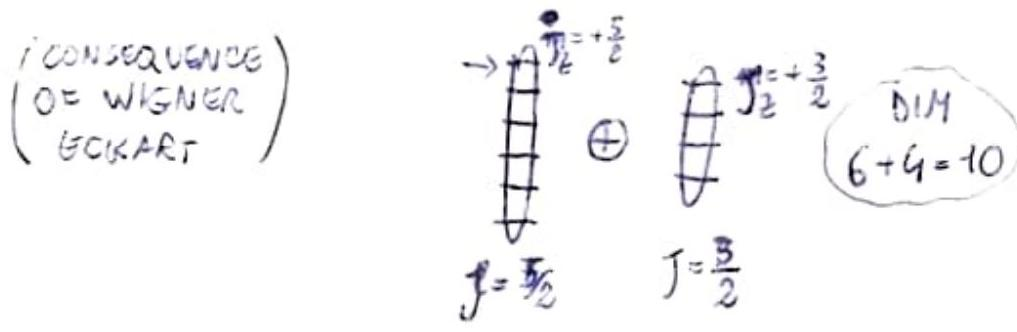
\includegraphics[max width=\textwidth, center]{2025_10_16_e34e240cf6beac2f9e0dg-4(1)}

$$
\begin{aligned}
& \text { FIXE) } \\
& \left|e^{\downarrow}, s, J, J_{z}\right\rangle=\sum\left(\mid e, m \cdot s, s^{z}\right) C_{e, m, m, s, n}^{\nu} \\
& \left|J_{1} J_{2}\right\rangle=\sum_{\left.m, s^{z}=J_{z}-m, s^{z}\right\rangle} \mid m s_{z}
\end{aligned}
$$

IT IS EASY TO FIND $\left|J_{\text {NAT }}, J_{\text {MAX }}\right\rangle=\left|e^{+} 5, e^{+}+5\right\rangle$\\
RECAUSE $\quad|j=l+5, j=l+5\rangle=\underset{\text { CHUCE }}{\text { +1 }} \quad\left|m=l, S_{z}=+5\right\rangle$\\
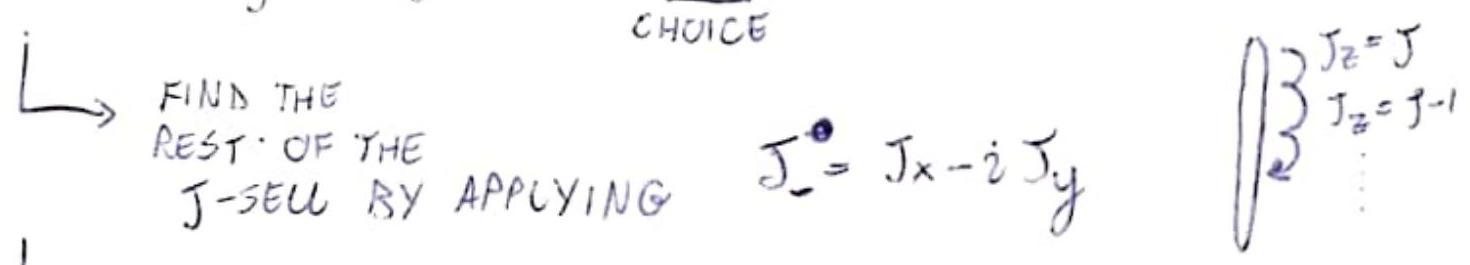
\includegraphics[max width=\textwidth, center]{2025_10_16_e34e240cf6beac2f9e0dg-4(2)}

THEN \$\textbackslash left.\textbackslash longrightarrow \textbackslash begin\{array\}\{c\}\text{FIND THE OTHER} \\
\\
\text{J-SHEU (S) BY} \\


\text{ORTMOGONALIZING}\textbackslash end\{array\}\textbackslash right\} \textbackslash quad\$\begin{tabular}{r}
$\left|J=l+S-1, J_{z}=l+S-1\right\rangle$ \\
$\mid S$ ORTHOCONAL TO \\
$\left|J=l+S, J_{z}=l-S-1\right\rangle$ \\
\end{tabular}$\quad$\begin{tabular}{r}
$|N S| \Delta E$ THE SDACE \\
$|m=l, S=S-1\rangle$, \\
$|m=l-1, S z=S\rangle$ \\
\end{tabular}

$\rightarrow$ eventuately repeat\\
(NOT NEEDES FOR $s=1 / 2$ )

$$
\begin{aligned}
& H_{\text {SFAN }}=(\operatorname{STUEF}(r)) \vec{S} \cdot \vec{L} \text { AND } \\
& (\vec{S}+\vec{L})^{2}=J^{2}=S^{2}+L^{2}+\frac{\vec{S} \cdot \vec{L}+L \cdot \vec{S}}{2 \vec{S} \cdot \vec{L}} \quad \vec{S} \cdot \vec{L}=\frac{1}{2}\left(J^{2}-L^{2}-S^{2}\right)
\end{aligned}
$$

$\left.\begin{array}{c}\text { arst order } \\ \text { perturbation }\end{array}\right\} \quad H^{(1)}=\pi_{\text {ne }} H_{\begin{array}{c}\text { spin } \\ \text { orbit }\end{array}} \Pi_{\text {ne }} \quad$ precisely $\quad\binom{\text { siagonal in }}{\text { esjfe }}$

$$
\begin{aligned}
& \Delta E_{\text {sprin }}=\left\langle n e_{j j_{2}}\right| H_{\text {onis }}\left|n e_{j j_{2}}\right\rangle \\
& =\frac{\mu_{s}\left(g_{s}-1\right) \hbar}{2 m c^{2} e}\left\langle n, \left.e_{1}\left(\frac{1}{\eta} \frac{\partial V_{s}}{\partial \eta}\right) \right\rvert\, n, l\right\rangle \underbrace{(J(j+1)}_{\text {POSITIVE }}-\underbrace{\left.\ell(l+1)-\frac{3}{4}\right)}_{\text {SAIT }}
\end{aligned}
$$

Sticl aegenerate in Te

$$
\begin{array}{ll}
l=l+1 / 2 & \operatorname{cose} \frac{U P}{N} \\
\underline{T=l-1 / 2} & \operatorname{coses} \frac{X O W}{N} \\
\hline & \text { in } E N \in R G Y
\end{array}
$$

LABELING LEVELS\\
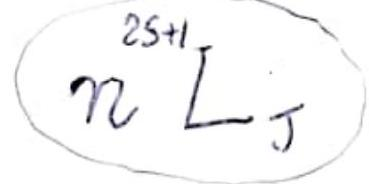
\includegraphics[width=0.5\textwidth, center]{2025_10_16_e34e240cf6beac2f9e0dg-5(1)}

FOR HYARCHKE $25+1$ is Always 2\\
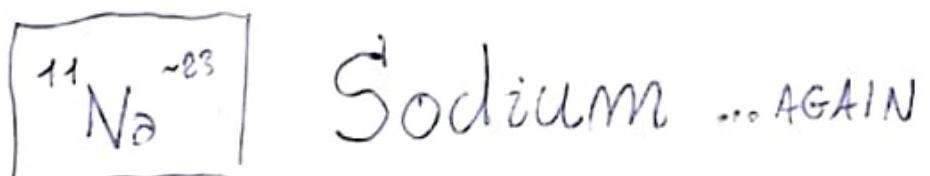
\includegraphics[width=0.5\textwidth, center]{2025_10_16_e34e240cf6beac2f9e0dg-5}

\begin{figure}[h]
\begin{center}
  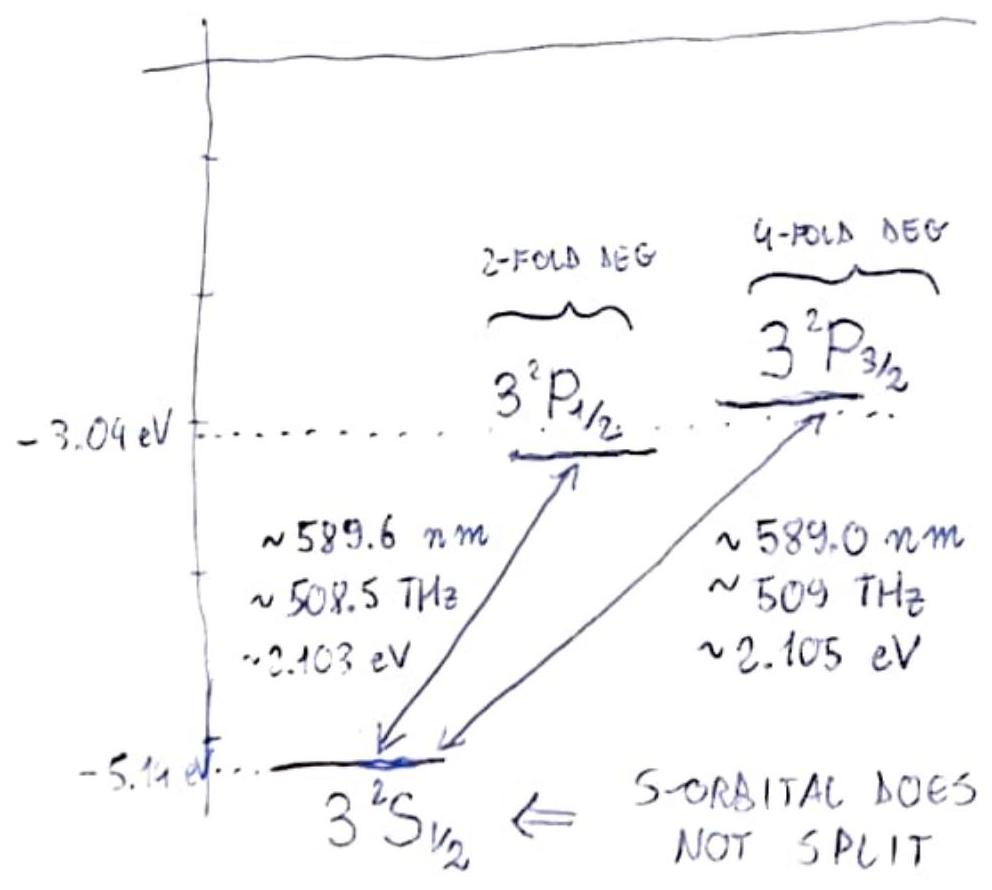
\includegraphics[width=\textwidth]{2025_10_16_e34e240cf6beac2f9e0dg-5(2)}
\captionsetup{labelformat=empty}
\caption{EMISSION/ABSORPTION SAECTRUM}
\end{center}
\end{figure}

\begin{figure}[h]
\begin{center}
\captionsetup{labelformat=empty}
\caption{EMISSION/ABSORPTION SAECTRUM}
  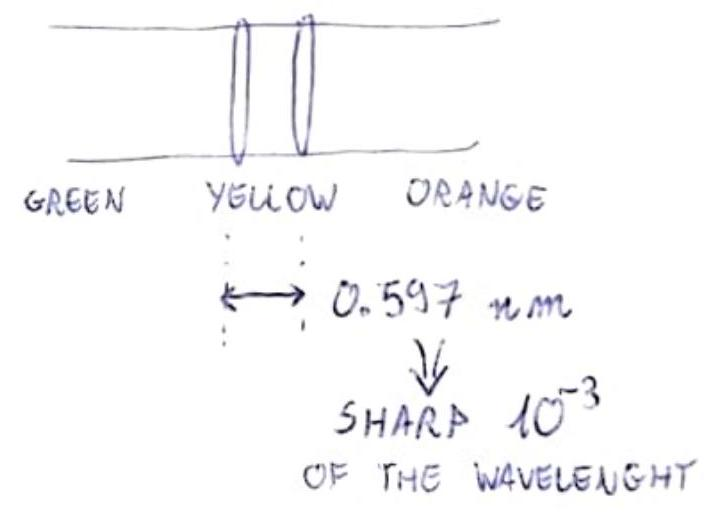
\includegraphics[width=\textwidth]{2025_10_16_e34e240cf6beac2f9e0dg-5(3)}
\end{center}
\end{figure}

at this energyscale there are hiso relativistic effects that SHIFT In es RIGIACY. BORNG.

$$
\begin{aligned}
& \text { External, Static Magnetic Fields } \\
& \vec{B} \text { UNIFORH, CONTANT, } \\
& \text { ruasical } \\
& H_{B}=-\vec{\mu}_{s} \cdot \vec{B}-\mu_{L} \cdot \vec{B}=\frac{\mu_{B}}{\hbar}\left(g_{s} \vec{S}+g_{L} \vec{L}\right) \cdot \vec{B} \\
& \begin{array}{l}
\text { SPIN HAGNETIC } \\
\text { OREITALE HAMENT DIPOLE HOMETIC } \\
\text { SIPONT }
\end{array} \\
& \text { DIPOLE HOMENT DIPOLE MOMENT } \\
& g \text {-FACTORS }\left\{\begin{array}{l}
g_{5} \quad \text { SOIN } \quad \text { giaction } \\
g_{c} \quad \text { ORBITAL } \quad g-\text { FACTIOR }=2,0023 \\
\frac{m c}{m_{e}}=\frac{1}{1+m_{e} / m_{\text {CORE }}} \approx 1-\varepsilon
\end{array}\right. \\
& \frac{\text { ROTATE }}{\text { UNTL B1S }} \\
& \text { AUGNCS ACONG } \hat{z} \\
& H_{B}=\frac{\mu_{B}}{\hbar}\left(\sim 2 \xi_{z}+\sim 1 L_{z}^{\infty}\right) B_{z} \quad\binom{\text { TO} D O S}{\text { SLEANRIOS }} \\
& 11 \begin{array}{c}
\text { strong } \\
\text { fields }
\end{array} \\
& \Delta E_{B} \gg \Delta E_{S A I N-O R S I T} \\
& \text { B~1 Tesla } \\
& \text { PASCHEN-BACK eff. } \\
& \text { at this energyscale, ( } m, s_{2} \text { ) are "goos" quantem nuhaers } \\
& \Delta E_{n l m s_{z}}=\left\langle n l m s_{z}\right| H_{B}\left|n l m s_{z}\right\rangle \cong \frac{\mu_{B} B}{\hbar}\left\langle 2 S_{z}+L_{z}\right\rangle
\end{aligned}
$$

$\begin{aligned} & 2 \text { weak } \\ & \text { Zeeman }\end{aligned}$\\
$\Delta E_{B} \backsim \Delta E_{\substack{\text { SPIN } \\ \text { ORBIT }}}$\\
$|n e, j, j z\rangle$\\
at this energyscale, good guantem numbers?\\
wer $\hat{A}_{n}$ elgenuection or $S_{z}$

HOW TO CACCULATE $\left\langle S_{z}\right\rangle$ WE USE THE\\
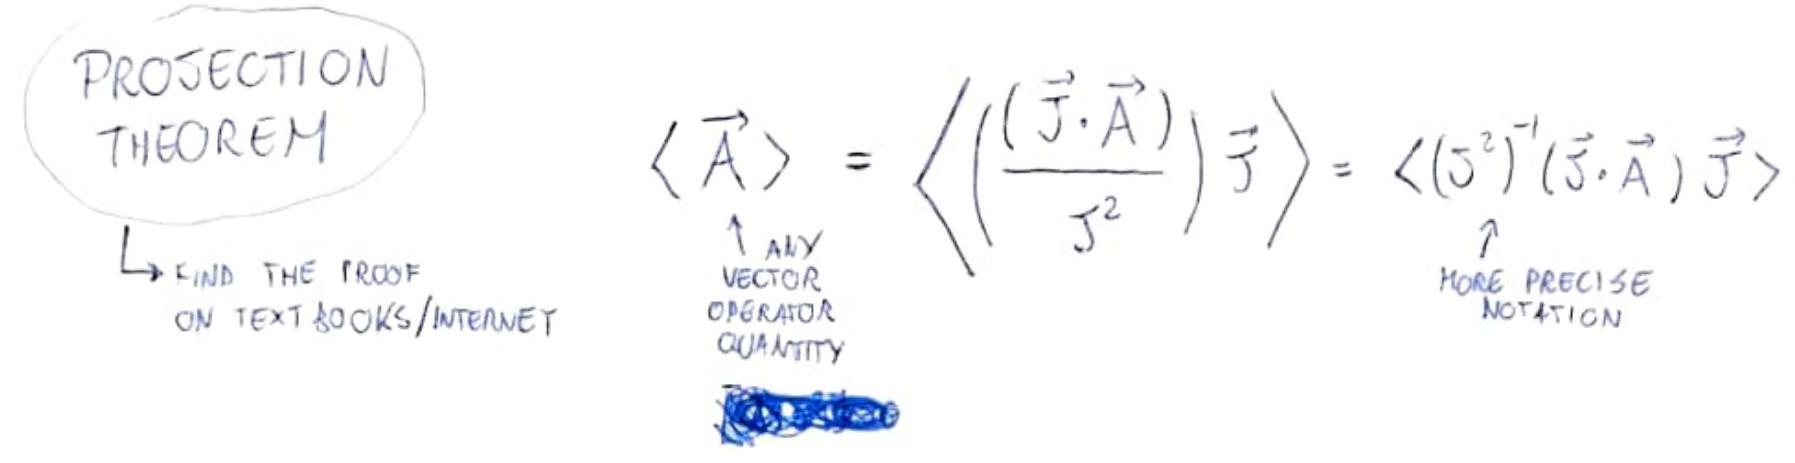
\includegraphics[width=0.5\textwidth, center]{2025_10_16_e34e240cf6beac2f9e0dg-7(2)}

$$
\begin{aligned}
\left\langle n l_{J J_{z}}\right| S_{z}\left|n l_{J J_{z}}\right\rangle & =\left\langle n l_{J J_{z}}\right|\left(J^{2}\right)^{-1}(\vec{J} \cdot \vec{S}) J_{z}\left|n l_{J J_{z}}\right\rangle= \\
& =\frac{J_{z}}{\hbar J_{J+1}}\left\langle n l_{J J_{z}}\right| \vec{J} \cdot \vec{S}\left|n l_{J J_{z}}\right\rangle
\end{aligned}
$$

$$
\begin{array}{ll}
\text { BUT } \vec{L}=\vec{J}-\vec{S} \text { so } & \Rightarrow \vec{J} \cdot \vec{S}=\frac{J^{2}+S^{2}-L^{2}}{2} \\
\left\langle x l_{j}=J^{2}+S^{2}-2\right| S_{z}\left|x l_{j} \vec{J} \cdot \vec{S}\right\rangle & \Rightarrow \frac{J(j+1)+s(S+1)-l(l+1)}{2 J(J+1)} J_{z} \hbar
\end{array}
$$

in conclusion $\Delta E_{n l j J_{z}}=+\mu_{B} J_{z} g_{f}(\tau, l) B_{z}$ where

$$
\underbrace{g_{J}^{(l, J)}}_{\substack{\text { LASEV } \\ g_{j}=\forall A C T O R}}=g_{L}+\left(g_{S}-g_{L}\right) \frac{j(J+1)-e(l+1)+\frac{3}{4}}{2 J(J+1)}
$$

LOW ORBITALS (EXEROISE)

$$
\begin{array}{ll}
S_{1 / 2} & g_{J} \approx 2 \approx g_{J} \\
P_{1 / 2} & g_{J} \approx \frac{2}{3} \\
P_{3 / 2} & g_{J} \approx \frac{4}{3}
\end{array}
$$

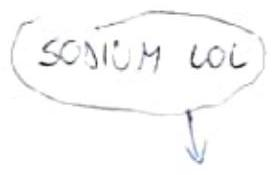
\includegraphics[width=0.5\textwidth, center]{2025_10_16_e34e240cf6beac2f9e0dg-7}\\
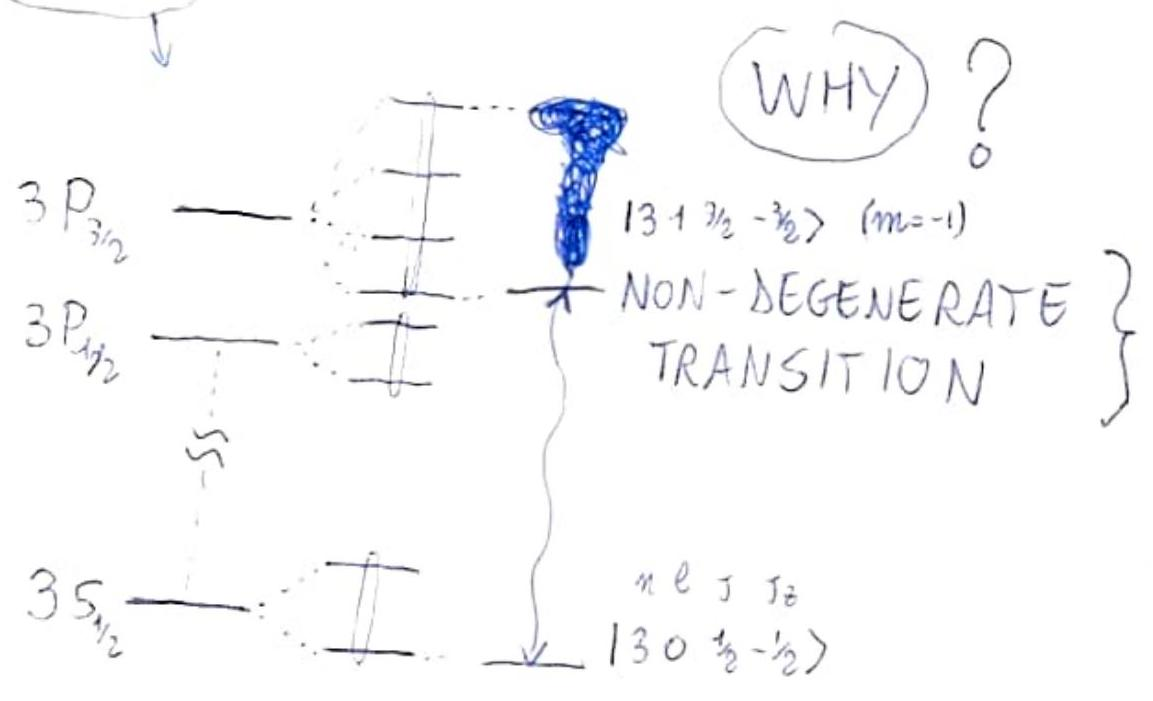
\includegraphics[width=0.5\textwidth, center]{2025_10_16_e34e240cf6beac2f9e0dg-7(1)}

THIS CAN BE AN AIOM $\frac{\text { QUBIT }}{\downarrow}$ DYNAMIC IS CONTROUES BY LIGHT W/ ELECTRIC DIPOLE TRANSITIONS\\
... speaking of allowed transimons, it is important to review the Dipole transition selection rules at the fine-structure ENERGYSCALE

\begin{center}
\begin{tabular}{ll}
$\left|n e^{-} S_{z} S_{z}\right\rangle$ & $\left|n e_{j} J_{z}\right\rangle$ \\
BAD QUANTUM NUMBERS & GOOD QUANUM NUMBERS \\
\end{tabular}
\end{center}

HYDROGEN-LIKE\\
ELECTRIC DIPOLE\\
(0) $\Delta l= \pm 1$\\
(2) $\triangle M n=0,4-1$ nore, $m$ is not a goos quantum number\\
(v) $\Delta J=0, \pm 1$ EXCEPT $J=J^{\prime}=0$\\
(v) $\Delta J_{z}=0, \pm 1$ BUT $\Delta_{J_{z}} \neq 0$ WLEN $\mathrm{J}=\mathrm{J}^{\prime}$

A the new rules come from the wigner-eckart theorem, THE PROOF IS TEDIOUS AND LONG.
